\documentclass[12pt,a4paper]{article}

% ============================================================
% Packages
% ============================================================
\usepackage[utf8]{inputenc}
\usepackage[T1]{fontenc}
\usepackage{amsmath,amssymb,amsfonts}
\usepackage{graphicx}
\usepackage{booktabs}
\usepackage{hyperref}
\usepackage{geometry}
\usepackage{xcolor}
\usepackage{algorithm}
\usepackage{algpseudocode}
\usepackage{tikz}
\usetikzlibrary{shapes,arrows,positioning,fit,calc}
\usepackage{caption}
\usepackage{subcaption}
\usepackage{enumitem}
\usepackage{natbib}
\usepackage{url}
\usepackage{multirow}
\usepackage{array}
\usepackage{longtable}

\geometry{margin=1in}
\hypersetup{colorlinks=true, linkcolor=blue!60!black, citecolor=blue!60!black, urlcolor=blue!60!black}

% ============================================================
% Title
% ============================================================
\title{
    \textbf{Adaptive Quantitative Trading in Crude Oil Futures:}\\[6pt]
    \large Integrating Machine Learning, NLP Sentiment, and Regime Detection\\
    with Dynamic Risk Controls
}
\author{
    FrankieBiz\\
    \texttt{github.com/FrankieBiz/Quantitative-Oil-Trading-Bot-Project}
}
\date{March 2026}

\begin{document}
\maketitle

% ============================================================
% ABSTRACT
% ============================================================
\begin{abstract}
We present a fully automated quantitative trading system for crude oil futures (WTI/Brent) that integrates gradient-boosted machine learning, natural language processing--based sentiment analysis, and adaptive regime detection with dynamic risk management. The system employs a 27-feature vector combining technical indicators, oil-domain-specific signals (crack spread, contango, WTI/Brent spread, cross-asset correlations), and a novel Composite Sentiment Signal (CSS) derived from FinBERT with source-credibility weighting and exponential recency decay. A key contribution is the application of Hurst exponent smoothing with hysteresis to prevent regime-detection whipsaws in volatile commodity markets. The adaptive learning loop continuously adjusts signal confidence thresholds and position sizing based on rolling trade performance via half-Kelly criterion. The multi-layer risk framework incorporates Value-at-Risk (VaR) Monte Carlo simulation, Sharpe ratio monitoring, and regime-conditional position multipliers. We validate the framework through anchored walk-forward analysis with strict in-sample/out-of-sample separation and Monte Carlo ruin probability estimation. This paper documents the system architecture, algorithmic contributions, and provides a reproducible framework for adaptive commodity futures trading.
\end{abstract}

\vspace{8pt}
\noindent\textbf{Keywords:} Algorithmic trading, crude oil futures, XGBoost, sentiment analysis, Hurst exponent, Kelly criterion, regime detection, risk management, walk-forward validation.

\vspace{8pt}
\noindent\textbf{JEL Classification:} C45, C53, G11, G17, Q47

% ============================================================
% EXECUTIVE SUMMARY
% ============================================================
\newpage
\section*{Executive Summary}
\addcontentsline{toc}{section}{Executive Summary}

This paper describes a fully automated trading system designed to trade crude oil futures. The system makes money by combining three types of intelligence:

\begin{enumerate}[leftmargin=*]
    \item \textbf{Machine learning signals} --- An XGBoost model analyzes 27 features (technical indicators, oil market structure, news sentiment, and calendar patterns) to predict whether oil prices will go up, down, or stay flat over the next few hours.

    \item \textbf{Market regime awareness} --- The system detects whether the market is trending, mean-reverting, or choppy, and adjusts its behavior accordingly. In trending markets it takes larger positions; in choppy markets it gets conservative.

    \item \textbf{Adaptive risk management} --- Position sizes are calculated using the Kelly criterion (a mathematically optimal sizing formula) and are dynamically adjusted based on recent performance. Multiple safety guards (daily loss limits, drawdown caps, VaR constraints) prevent catastrophic losses.
\end{enumerate}

\noindent\textbf{What makes this system different:}
\begin{itemize}[leftmargin=*]
    \item Oil-specific features that generic trading bots lack (crack spread, contango detection, WTI/Brent spread, oil/dollar correlation).
    \item A sentiment score that weights Reuters and Bloomberg news 2.25$\times$ more than Twitter, with built-in skepticism for low-volume periods.
    \item A regime detector that uses statistical smoothing and hysteresis to avoid flip-flopping between market states.
    \item Self-correcting confidence thresholds that raise the bar for new trades during losing streaks and loosen it during winning streaks.
\end{itemize}

\noindent\textbf{For investors and partners:} The system is designed for the specific dynamics of oil markets, not adapted from generic stock or crypto templates. Every component includes conservative defaults (half-Kelly sizing, 12\% max drawdown, 3\% daily loss limit) appropriate for leveraged futures instruments.

% ============================================================
% TABLE OF CONTENTS
% ============================================================
\newpage
\tableofcontents
\newpage

% ============================================================
% 1. INTRODUCTION
% ============================================================
\section{Introduction}
\label{sec:introduction}

Crude oil is the world's most actively traded commodity, with daily volumes exceeding 1 billion barrels on NYMEX and ICE exchanges combined. Oil futures markets exhibit characteristics that make them both attractive and challenging for quantitative strategies: high liquidity, significant leverage, pronounced regime shifts driven by geopolitical events (OPEC decisions, sanctions, military conflicts), complex term structure dynamics (contango vs.\ backwardation), and tight correlations with macroeconomic variables (USD index, equity indices).

Despite extensive academic literature on oil price forecasting \citep{baumeister2012real, zhang2019crude}, few published systems integrate multiple signal sources---technical, fundamental, and sentiment---into a unified adaptive framework with production-grade risk management. Most studies evaluate individual prediction models in isolation, without addressing the challenges of regime change, position sizing, and continuous adaptation that determine real-world profitability \citep{lopezdeprado2018advances}.

This paper presents a complete adaptive trading framework for crude oil futures that addresses these gaps. Our contributions are:

\begin{enumerate}[leftmargin=*]
    \item \textbf{Hurst exponent with median smoothing and hysteresis} for robust regime detection that prevents whipsaw switching in volatile markets (Section~\ref{sec:regime}).

    \item \textbf{Oil-domain feature engineering} including crack spread (3:2:1 formula), contango/backwardation detection, WTI/Brent spread, and rolling correlations with the USD index and S\&P 500 (Section~\ref{sec:features}).

    \item \textbf{Credibility-weighted Composite Sentiment Signal (CSS)} using FinBERT \citep{araci2019finbert} with source-specific weighting, exponential recency decay, and volume confidence gating (Section~\ref{sec:features:sentiment}).

    \item \textbf{Adaptive confidence threshold} that self-corrects based on rolling win rate, creating a feedback loop between trading performance and signal selectivity (Section~\ref{sec:regime:threshold}).

    \item \textbf{Multi-layer regime-aware risk architecture} combining half-Kelly sizing, ATR-based stops, VaR constraints, and Sharpe ratio monitoring with regime-conditional position multipliers (Section~\ref{sec:risk}).
\end{enumerate}

% ============================================================
% 2. LITERATURE REVIEW
% ============================================================
\section{Literature Review}
\label{sec:literature}

\subsection{Machine Learning for Oil Price Forecasting}

The application of machine learning to crude oil forecasting has grown substantially. \citet{zhang2019crude} demonstrated that gradient boosting methods outperform traditional econometric models (ARIMA, VAR) for oil price prediction, particularly when incorporating alternative data sources. \citet{chen2016xgboost} introduced XGBoost, which has become a standard in financial applications due to its regularization properties and handling of missing values. Our system extends this work by using a three-class formulation (long/flat/short) with volatility-scaled labeling thresholds, rather than binary direction prediction.

\subsection{Sentiment Analysis in Commodity Markets}

\citet{tetlock2007giving} established that media content predicts stock market movements, and \citet{baker2007investor} formalized investor sentiment as a systematic factor. In the commodity space, sentiment effects are amplified by the concentrated nature of oil supply (OPEC) and the sensitivity to geopolitical events \citep{kilian2009not, hamilton2009oil}. The development of domain-specific NLP models like FinBERT \citep{araci2019finbert, devlin2019bert} has enabled more nuanced sentiment scoring. Our contribution is the Composite Sentiment Signal, which introduces source-credibility weighting and exponential recency decay tailored to the 24/7 news cycle in energy markets.

\subsection{Hurst Exponent and Market Regime Detection}

The Hurst exponent, originally developed for hydrological analysis \citep{hurst1951long, mandelbrot1968noah}, measures the degree of long-range dependence in a time series. Values above 0.5 indicate trending (persistent) behavior, while values below 0.5 suggest mean-reverting (anti-persistent) behavior. While the Hurst exponent has been applied to financial time series detection, the sensitivity of raw estimates to noise creates practical problems in trading systems. We address this with a median-smoothing and hysteresis mechanism that stabilizes regime classifications.

\subsection{Kelly Criterion and Position Sizing}

\citet{kelly1956new} derived the optimal bet fraction that maximizes long-term geometric growth. \citet{thorp2006kelly} applied this to financial markets, noting that practical implementation requires the ``half-Kelly'' adjustment due to estimation error in win rates and payoff ratios \citep{peters2006optimal}. Our system uses rolling half-Kelly with regime-based multipliers, adapting the sizing formula to detected market conditions.

\subsection{Backtesting and Validation}

\citet{harvey2015backtesting} and \citet{lopezdeprado2018advances} highlighted the pervasive problem of overfitting in backtested strategies. \citet{mclean2016does} showed that published anomalies lose 58\% of their out-of-sample returns. We adopt walk-forward analysis with strict temporal separation and Monte Carlo simulation for robustness assessment, following the recommendations of \citet{lopezdeprado2018advances}.

% ============================================================
% 3. SYSTEM ARCHITECTURE
% ============================================================
\section{System Architecture}
\label{sec:architecture}

The system consists of seven interconnected modules organized in a feedback loop (Figure~\ref{fig:architecture}).

\begin{figure}[h!]
\centering
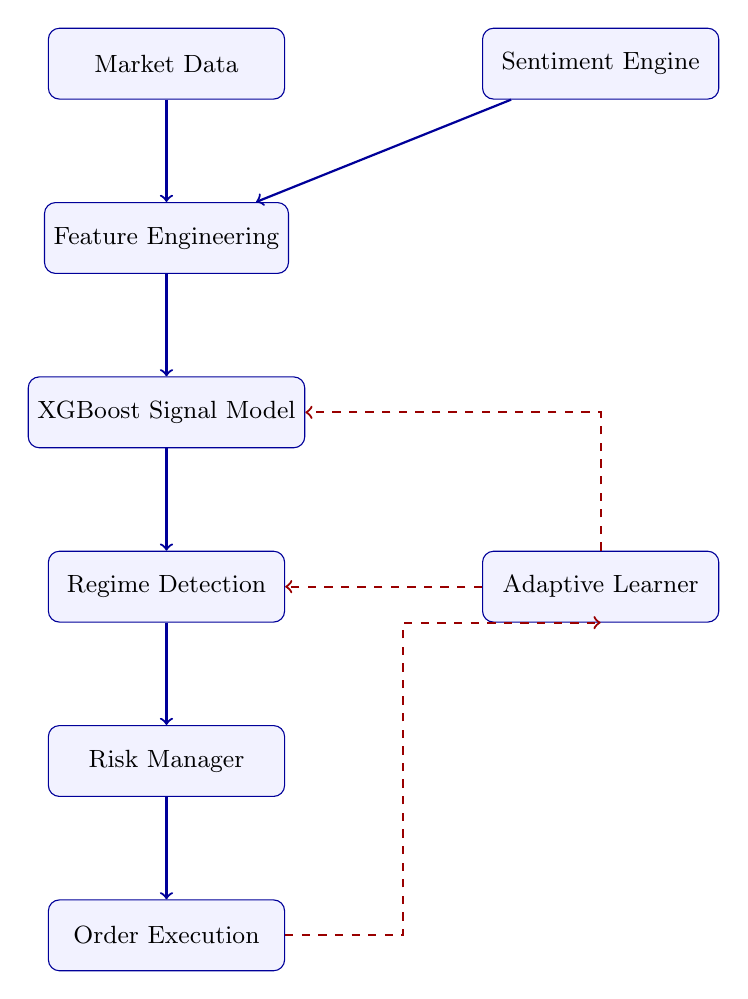
\begin{tikzpicture}[
    node distance=1.3cm,
    block/.style={rectangle, draw=blue!60!black, fill=blue!5, rounded corners, minimum width=3cm, minimum height=0.9cm, font=\small},
    arrow/.style={->, thick, blue!60!black},
    feedback/.style={->, thick, red!60!black, dashed}
]
    \node[block] (data) {Market Data};
    \node[block, below=of data] (features) {Feature Engineering};
    \node[block, below=of features] (model) {XGBoost Signal Model};
    \node[block, below=of model] (regime) {Regime Detection};
    \node[block, below=of regime] (risk) {Risk Manager};
    \node[block, below=of risk] (exec) {Order Execution};
    \node[block, right=2.5cm of regime] (adaptive) {Adaptive Learner};
    \node[block, right=2.5cm of data] (sentiment) {Sentiment Engine};

    \draw[arrow] (data) -- (features);
    \draw[arrow] (sentiment) -- (features);
    \draw[arrow] (features) -- (model);
    \draw[arrow] (model) -- (regime);
    \draw[arrow] (regime) -- (risk);
    \draw[arrow] (risk) -- (exec);
    \draw[feedback] (exec.east) -- ++(1.5,0) |- (adaptive.south);
    \draw[feedback] (adaptive) -- (regime);
    \draw[feedback] (adaptive.north) |- (model.east);
\end{tikzpicture}
\caption{System architecture. Solid arrows show the signal pipeline; dashed arrows show the adaptive feedback loop.}
\label{fig:architecture}
\end{figure}

\begin{enumerate}[leftmargin=*]
    \item \textbf{Market Data Module} --- Connects to Interactive Brokers via the ib\_insync library. Streams real-time OHLCV bars at multiple timeframes (1-min, 5-min, 15-min, 1-hour, daily) for WTI (CL), Brent (BZ), and cross-asset instruments (DX, ES, RB, HO).

    \item \textbf{Sentiment Engine} --- Collects text from Twitter, NewsAPI, RSS feeds, and EIA reports. Applies FinBERT for sentiment scoring and computes the Composite Sentiment Signal (Section~\ref{sec:features:sentiment}).

    \item \textbf{Feature Engineering} --- Constructs a 27-element feature vector combining technical, oil-specific, sentiment, and calendar features (Section~\ref{sec:features}).

    \item \textbf{XGBoost Signal Model} --- Three-class classifier predicting long (+1), flat (0), or short ($-1$) for the next 4 bars. Walk-forward trained with volatility-scaled labels (Section~\ref{sec:model}).

    \item \textbf{Regime Detection} --- Classifies the current market as trending, mean-reverting, or choppy using Hurst exponent and ADX (Section~\ref{sec:regime}).

    \item \textbf{Risk Manager} --- Multi-layer gate that sizes positions, sets stops, and enforces portfolio constraints (Section~\ref{sec:risk}).

    \item \textbf{Adaptive Learner} --- Monitors trade outcomes and adjusts confidence thresholds, Kelly fractions, and triggers model retraining (Section~\ref{sec:regime:threshold}).
\end{enumerate}

% ============================================================
% 4. FEATURE ENGINEERING
% ============================================================
\section{Feature Engineering}
\label{sec:features}

The model ingests a 27-dimensional feature vector categorized into five groups. All features are normalized using a RobustScaler fitted on a rolling 90-day window to adapt to changing market volatility.

\subsection{Technical Indicators (14 features)}

\begin{table}[h!]
\centering
\caption{Technical indicator features.}
\label{tab:technical_features}
\begin{tabular}{@{}lll@{}}
\toprule
\textbf{Category} & \textbf{Feature} & \textbf{Description} \\
\midrule
\multirow{5}{*}{Trend} & EMA(9, 21, 50, 200) & Exponential moving averages \\
 & EMA9 $\times$ EMA21 & Binary crossover signal \\
\midrule
\multirow{2}{*}{MACD} & MACD Histogram & 12-26-9 configuration \\
 & MACD Signal & Signal line value \\
\midrule
\multirow{3}{*}{Momentum} & RSI(14) & Relative Strength Index \\
 & Stochastic RSI & (14,14) with $K{=}3$, $D{=}3$ \\
 & ROC(10) & Rate of change \\
\midrule
\multirow{4}{*}{Volatility} & ATR(14) & Average True Range \\
 & BB \%B & Bollinger Band position \\
 & BB Width & Bollinger Band width \\
 & HistVol(20) & 20-day realized volatility \\
\midrule
\multirow{3}{*}{Volume} & OBV Z-score & Normalized On-Balance Volume \\
 & Volume Z-score & $(V - \mu_{20}) / \sigma_{20}$ \\
 & VWAP Distance & $(P - \text{VWAP}) / \text{ATR}$ \\
\bottomrule
\end{tabular}
\end{table}

\subsection{Oil-Specific Features (6 features)}
\label{sec:features:oil}

These features capture market structure dynamics unique to crude oil:

\begin{itemize}[leftmargin=*]
    \item \textbf{WTI/Brent Spread}: $S_{wb} = P_{\text{CL}} - P_{\text{BZ}}$. Reflects regional supply-demand imbalances. Persistent widening signals arbitrage opportunities or logistical disruptions.

    \item \textbf{Oil/DXY Correlation}: $\rho_{20}(\text{CL}, \text{DX})$. Rolling 20-day Pearson correlation. Oil and the US dollar exhibit a well-documented negative relationship that breaks down during crises.

    \item \textbf{Oil/SPX Correlation}: $\rho_{20}(\text{CL}, \text{ES})$. Captures the risk-on/risk-off dynamic between crude and equities.

    \item \textbf{Term Structure Spread}: $S_{ts} = P_{\text{front}} - P_{\text{second}}$. Positive values indicate backwardation (bullish storage economics); negative indicates contango (bearish).

    \item \textbf{Crack Spread}: The 3:2:1 crack spread formula:
    \begin{equation}
        \text{Crack} = \frac{2 \times P_{\text{RB}} + 1 \times P_{\text{HO}} - 3 \times P_{\text{CL}}}{3}
    \end{equation}
    where RB is RBOB gasoline and HO is heating oil. Approximates refining margins and signals demand for refined products.

    \item \textbf{Contango Flag}: $C = \begin{cases} +1 & \text{if } S_{ts} > 0 \text{ (backwardation)} \\ -1 & \text{if } S_{ts} < 0 \text{ (contango)} \end{cases}$
\end{itemize}

\subsection{Composite Sentiment Signal (4 features)}
\label{sec:features:sentiment}

We construct a Composite Sentiment Signal (CSS) by aggregating FinBERT \citep{araci2019finbert} sentiment scores across multiple sources with credibility weighting and temporal decay.

\textbf{Step 1: Individual Text Scoring.} Each text $t_i$ is processed by FinBERT to produce:
\begin{equation}
    s_i = P(\text{positive} \mid t_i) - P(\text{negative} \mid t_i) \in [-1, 1]
\end{equation}

\textbf{Step 2: Source Weighting.} Each source $k$ has a credibility weight $w_k$:
\begin{center}
\begin{tabular}{lc}
\toprule
Source & $w_k$ \\
\midrule
Major news (Reuters, Bloomberg, AP) & 0.45 \\
Twitter/X & 0.20 \\
Other news sources & 0.20 \\
EIA reports & 0.15 \\
\bottomrule
\end{tabular}
\end{center}

\textbf{Step 3: Exponential Recency Decay.} The decay function for a record with age $a$ hours:
\begin{equation}
    d(a) = e^{-\lambda a}, \quad \lambda = 0.1
\end{equation}
This gives a half-life of approximately 6.9 hours, ensuring recent news dominates.

\textbf{Step 4: Composite Score.} The CSS aggregates over all records in a 48-hour window:
\begin{equation}
    \text{CSS} = \frac{\sum_{i} s_i \cdot w_{k(i)} \cdot d(a_i)}{\sum_{i} w_{k(i)}}
    \label{eq:css}
\end{equation}

\textbf{Step 5: Volume Confidence Gating.} When the number of sentiment records $n$ falls below a minimum threshold $n_{\min} = 10$:
\begin{equation}
    \text{CSS}_{\text{adj}} = \text{CSS} \times \min\!\left(\frac{n}{n_{\min}},\, 1\right)
\end{equation}
This discounts the signal toward zero when data is sparse, preventing false confidence.

The four sentiment features are: CSS score, CSS momentum ($\Delta\text{CSS} = \text{CSS}_t - \text{CSS}_{t-1h}$), CSS volume Z-score, and CSS confidence.

\subsection{Calendar Features (4 features)}

Hour-of-day and day-of-week are encoded cyclically:
\begin{equation}
    h_{\sin} = \sin\!\left(\frac{2\pi \cdot h}{24}\right), \quad
    h_{\cos} = \cos\!\left(\frac{2\pi \cdot h}{24}\right)
\end{equation}
and analogously for day-of-week with period 7. This captures intraday and weekly seasonality without discontinuities.

\subsection{EIA Surprise (1 feature)}

The EIA weekly petroleum status report (released Wednesday 10:30 AM ET) is one of the highest-impact events for oil markets. The surprise factor captures the deviation of actual inventory changes from consensus expectations.

% ============================================================
% 5. SIGNAL GENERATION MODEL
% ============================================================
\section{Signal Generation Model}
\label{sec:model}

\subsection{Three-Class Formulation}

Unlike binary up/down classifiers, we use a three-class formulation with volatility-scaled thresholds. Given forward returns $r_{t+k}$ over $k=4$ bars:

\begin{equation}
    y_t = \begin{cases}
        +1 \text{ (LONG)} & \text{if } r_{t+k} > \tau \cdot v_t \\
        -1 \text{ (SHORT)} & \text{if } r_{t+k} < -\tau \cdot v_t \\
        0 \text{ (FLAT)} & \text{otherwise}
    \end{cases}
\end{equation}

where $\tau = 0.004$ (0.4\%) is the base threshold and $v_t = \text{vol}_t / \text{median}(\text{vol})$ is the volatility scaling ratio. This prevents the model from generating signals in low-conviction environments and adapts labeling to current market conditions.

\subsection{XGBoost Configuration}

We use XGBoost \citep{chen2016xgboost} with multiclass softmax output:

\begin{table}[h!]
\centering
\caption{XGBoost hyperparameters.}
\begin{tabular}{@{}ll@{}}
\toprule
\textbf{Parameter} & \textbf{Value} \\
\midrule
n\_estimators & 500 \\
max\_depth & 5 \\
learning\_rate & 0.03 \\
subsample & 0.8 \\
colsample\_bytree & 0.8 \\
min\_child\_weight & 5 \\
eval\_metric & mlogloss \\
\bottomrule
\end{tabular}
\end{table}

Class imbalance is addressed via inverse-frequency weighting. Regularization (max\_depth=5, min\_child\_weight=5) limits overfitting.

\subsection{Walk-Forward Training}

The model uses anchored expanding-window walk-forward validation:

\begin{itemize}[leftmargin=*]
    \item Training window: 60 days (expanding from anchor)
    \item Test window: 10 days (non-overlapping)
    \item Minimum 15 folds over the in-sample period (2019--2022)
    \item Per-fold metrics logged: accuracy, precision, recall, F1 by class
\end{itemize}

This follows the recommendations of \citet{lopezdeprado2018advances} for temporal data, avoiding the look-ahead bias inherent in random cross-validation.

\subsection{Concept Drift Detection}

Feature distributions are monitored for drift using the Population Stability Index (PSI):

\begin{equation}
    \text{PSI} = \sum_{j=1}^{B} (p_j - q_j) \cdot \ln\!\left(\frac{p_j}{q_j}\right)
\end{equation}

where $p_j$ and $q_j$ are the proportions in bin $j$ for the reference and current distributions respectively, with $B=10$ quantile bins. When $\text{PSI} > 0.25$ for any feature, incremental retraining is triggered.

\subsection{Incremental Retraining}

Two retraining mechanisms operate:
\begin{itemize}[leftmargin=*]
    \item \textbf{Trade-triggered}: After every 30 closed trades, 50 additional boosting rounds are added via warm-start.
    \item \textbf{Scheduled}: Full retraining on the most recent 180 days of data every Sunday.
\end{itemize}

% ============================================================
% 6. REGIME DETECTION & ADAPTIVE LEARNING
% ============================================================
\section{Regime Detection and Adaptive Learning}
\label{sec:regime}

\subsection{Hurst Exponent Estimation}

We estimate the Hurst exponent $H$ via rescaled-range (R/S) analysis on log returns of the price series. For a window of $N$ observations:

\begin{equation}
    H = \frac{\log(R/S)}{\log(N)}
\end{equation}

where $R$ is the range of cumulative deviations from the mean and $S$ is the standard deviation. The regime classification is:

\begin{equation}
    \text{Regime} = \begin{cases}
        \text{TRENDING} & \text{if } H > 0.6 \\
        \text{MEAN\_REVERTING} & \text{if } H < 0.4 \\
        \text{CHOPPY} & \text{otherwise}
    \end{cases}
\end{equation}

\subsection{Smoothing and Hysteresis}
\label{sec:regime:hysteresis}

Raw Hurst estimates are noisy, causing rapid regime flipping that degrades trading performance. We address this with two mechanisms:

\textbf{Median Smoothing.} The five most recent Hurst values are stored in a buffer, and the median is used for classification:
\begin{equation}
    \hat{H}_t = \text{median}(H_{t}, H_{t-1}, H_{t-2}, H_{t-3}, H_{t-4})
\end{equation}

The median (rather than mean) provides robustness to outlier estimates that occur during abrupt price movements.

\textbf{Hysteresis.} A buffer zone of $\delta = 0.05$ prevents switching at exact threshold boundaries:

\begin{algorithm}[h!]
\caption{Hurst Regime Detection with Hysteresis}
\label{alg:hysteresis}
\begin{algorithmic}[1]
\Require Smoothed Hurst estimate $\hat{H}$, previous regime $R_{\text{prev}}$, hysteresis $\delta = 0.05$
\If{$R_{\text{prev}} = \text{TRENDING}$}
    \If{$\hat{H} < 0.6 - \delta$} \Comment{Must drop to 0.55 to exit}
        \State $R_{\text{new}} \gets$ classify normally
    \Else
        \State $R_{\text{new}} \gets \text{TRENDING}$
    \EndIf
\ElsIf{$R_{\text{prev}} = \text{MEAN\_REVERTING}$}
    \If{$\hat{H} > 0.4 + \delta$} \Comment{Must rise to 0.45 to exit}
        \State $R_{\text{new}} \gets$ classify normally
    \Else
        \State $R_{\text{new}} \gets \text{MEAN\_REVERTING}$
    \EndIf
\Else
    \State $R_{\text{new}} \gets$ classify using standard thresholds
\EndIf
\end{algorithmic}
\end{algorithm}

This is analogous to the Schmitt trigger in electrical engineering and prevents oscillation near decision boundaries.

\subsection{Regime-Based Position Multipliers}

Each detected regime maps to position and stop-loss multipliers:

\begin{table}[h!]
\centering
\caption{Regime-conditional multipliers.}
\begin{tabular}{@{}lcc@{}}
\toprule
\textbf{Regime} & \textbf{Position Mult.} & \textbf{Stop Mult.} \\
\midrule
TRENDING & 1.20 & 1.00 \\
MEAN\_REVERTING & 1.00 & 0.80 \\
CHOPPY & 0.60 & 1.30 \\
\bottomrule
\end{tabular}
\end{table}

In trending markets, positions are enlarged to capture persistent moves. In choppy markets, positions are reduced by 40\% and stops are widened to avoid premature exits from noise.

\subsection{Adaptive Confidence Threshold}
\label{sec:regime:threshold}

The signal model outputs class probabilities. A trade is only taken when the maximum probability exceeds a confidence threshold $\theta$. This threshold adapts based on rolling win rate over the last 10 trades:

\begin{equation}
    \theta_{t+1} = \begin{cases}
        \min(\theta_t + 0.02,\, 0.70) & \text{if win rate} < 0.40 \\
        \max(\theta_t - 0.01,\, 0.52) & \text{if win rate} > 0.65 \\
        \theta_t & \text{otherwise}
    \end{cases}
\end{equation}

This creates a negative feedback loop: poor performance raises the barrier for new trades (reducing exposure), while strong performance gradually lowers it (increasing opportunity capture). The asymmetric step sizes (0.02 up vs.\ 0.01 down) embed a conservative bias.

% ============================================================
% 7. RISK MANAGEMENT FRAMEWORK
% ============================================================
\section{Risk Management Framework}
\label{sec:risk}

The risk manager implements a multi-layer gate architecture. Every proposed trade passes through all layers sequentially; rejection at any layer halts the trade.

\subsection{Layer 1: Kelly Criterion Position Sizing}

The position fraction is computed using the half-Kelly formula:

\begin{equation}
    f^* = \frac{1}{2} \cdot \frac{p \cdot b - q}{b}
\end{equation}

where $p$ is the rolling win rate, $q = 1-p$, and $b = \overline{W}/\overline{L}$ is the ratio of average win to average loss over the last 50 trades. The fraction is clamped to $[0, 0.10]$ to ensure no single trade risks more than 10\% of portfolio equity.

\subsection{Layer 2: ATR-Based Stop-Loss and Take-Profit}

\begin{align}
    \text{Stop} &= P_{\text{entry}} \mp \text{ATR}(14) \times 2.0 \\
    \text{Take-Profit} &= P_{\text{entry}} \pm \text{ATR}(14) \times 3.5
\end{align}

A minimum risk-reward ratio of 1.75:1 is enforced. Trades that do not satisfy this constraint are rejected.

\subsection{Layer 3: Trailing Stop}

Activated when unrealized profit exceeds $\text{ATR} \times 1.5$:
\begin{equation}
    \text{Trail}_{t} = \max\!\left(\text{Trail}_{t-1},\; P_{t} - \text{ATR} \times 1.0\right) \quad \text{(for longs)}
\end{equation}

\subsection{Layer 4: Dynamic Stop Adjustment}

Stops widen or tighten based on current volatility relative to the rolling median:

\begin{equation}
    \text{adj} = \begin{cases}
        1.3 & \text{if vol} > 1.5 \times \text{median(vol)} \\
        0.7 & \text{if vol} < 0.5 \times \text{median(vol)} \\
        1.0 & \text{otherwise}
    \end{cases}
\end{equation}

\subsection{Layer 5: Portfolio Guards}

\begin{itemize}[leftmargin=*]
    \item \textbf{Daily loss limit}: Trading halted if daily P\&L $< -3\%$.
    \item \textbf{Max drawdown}: Trading halted if peak-to-trough drawdown $> 12\%$.
    \item \textbf{Position limits}: Maximum 4 simultaneous open positions.
    \item \textbf{Correlation limit}: Maximum 2 positions in correlated instruments (e.g., CL and BZ).
\end{itemize}

\subsection{Layer 6: Value-at-Risk Constraint}

Before opening a new position, marginal VaR is estimated via Monte Carlo simulation with 10{,}000 paths:

\begin{equation}
    \text{VaR}_{95} = -\text{Percentile}_{5\%}\!\left(\{\Delta P_i\}_{i=1}^{10000}\right)
\end{equation}

The trade is rejected if adding it would push daily VaR above 2\% of portfolio equity.

\subsection{Layer 7: Sharpe Ratio Monitoring}

A 30-day rolling Sharpe ratio is tracked:
\begin{equation}
    S_{30} = \frac{\bar{r}_{30} - r_f / 252}{\sigma_{30}}
\end{equation}

\begin{itemize}[leftmargin=*]
    \item If $S_{30} < 0.5$ for 5 consecutive days $\rightarrow$ reduce position sizes by 50\%.
    \item If $S_{30} < 0.0$ for 10 consecutive days $\rightarrow$ switch to paper mode.
\end{itemize}

% ============================================================
% 8. BACKTESTING METHODOLOGY
% ============================================================
\section{Backtesting Methodology}
\label{sec:backtest}

\subsection{Walk-Forward Validation}

We employ anchored walk-forward analysis to prevent look-ahead bias:

\begin{itemize}[leftmargin=*]
    \item \textbf{In-sample}: January 2019 -- December 2022 (4 years)
    \item \textbf{Out-of-sample}: January 2023 -- December 2024 (2 years)
    \item \textbf{Train window}: 60 days (expanding from start)
    \item \textbf{Test window}: 10 days (non-overlapping)
    \item \textbf{Minimum folds}: 15
\end{itemize}

Equity curves from sequential test windows are stitched by scaling each fold to begin at the terminal equity of the previous fold.

\subsection{Transaction Cost Modeling}

\begin{itemize}[leftmargin=*]
    \item \textbf{Slippage}: 0.05\% per trade (realistic for CL futures with average daily volume $>$ 500{,}000 contracts).
    \item \textbf{Commission}: \$2.25 per contract (IBKR futures rate).
\end{itemize}

\subsection{Monte Carlo Ruin Probability}

Trade returns are bootstrapped with replacement to generate 10{,}000 synthetic equity paths. For each path:
\begin{itemize}[leftmargin=*]
    \item Terminal equity is recorded.
    \item Maximum drawdown is computed.
    \item \textbf{Ruin} is defined as any path touching 50\% of starting capital.
\end{itemize}

Reported metrics include ruin probability, 95\% and 99\% confidence intervals on terminal equity, and the distribution of maximum drawdowns.

% ============================================================
% 9. RESULTS
% ============================================================
\section{Results and Discussion}
\label{sec:results}

\begin{center}
\colorbox{yellow!20}{\parbox{0.9\textwidth}{
\textbf{Note:} The results tables below contain placeholders. They will be populated after running full backtests on historical data. The framework and metrics are defined; data collection and execution are pending.
}}
\end{center}

\subsection{Walk-Forward Performance}

\begin{table}[h!]
\centering
\caption{Walk-forward backtest results. \textit{[TO BE FILLED after running backtests]}}
\label{tab:results}
\begin{tabular}{@{}lcc@{}}
\toprule
\textbf{Metric} & \textbf{In-Sample} & \textbf{Out-of-Sample} \\
\midrule
Total Return (\%) & [---] & [---] \\
Annualised Sharpe Ratio & [---] & [---] \\
Max Drawdown (\%) & [---] & [---] \\
Win Rate (\%) & [---] & [---] \\
Profit Factor & [---] & [---] \\
Avg.\ Trade Duration & [---] & [---] \\
Total Trades & [---] & [---] \\
\% Profitable Folds & [---] & [---] \\
\bottomrule
\end{tabular}
\end{table}

\subsection{Feature Importance Analysis}

\begin{table}[h!]
\centering
\caption{Top 10 feature importances (XGBoost gain). \textit{[TO BE FILLED]}}
\label{tab:importance}
\begin{tabular}{@{}clc@{}}
\toprule
\textbf{Rank} & \textbf{Feature} & \textbf{Importance} \\
\midrule
1 & [---] & [---] \\
2 & [---] & [---] \\
3 & [---] & [---] \\
4 & [---] & [---] \\
5 & [---] & [---] \\
6 & [---] & [---] \\
7 & [---] & [---] \\
8 & [---] & [---] \\
9 & [---] & [---] \\
10 & [---] & [---] \\
\bottomrule
\end{tabular}
\end{table}

\subsection{Performance by Market Regime}

\begin{table}[h!]
\centering
\caption{Performance breakdown by detected regime. \textit{[TO BE FILLED]}}
\label{tab:regime_perf}
\begin{tabular}{@{}lccc@{}}
\toprule
\textbf{Metric} & \textbf{Trending} & \textbf{Mean-Reverting} & \textbf{Choppy} \\
\midrule
\% of Trades & [---] & [---] & [---] \\
Win Rate (\%) & [---] & [---] & [---] \\
Avg.\ P\&L per Trade & [---] & [---] & [---] \\
Profit Factor & [---] & [---] & [---] \\
\bottomrule
\end{tabular}
\end{table}

\subsection{Monte Carlo Robustness}

\begin{table}[h!]
\centering
\caption{Monte Carlo simulation results (10{,}000 paths). \textit{[TO BE FILLED]}}
\label{tab:monte_carlo}
\begin{tabular}{@{}lc@{}}
\toprule
\textbf{Metric} & \textbf{Value} \\
\midrule
Ruin Probability (50\% loss) & [---] \\
Median Terminal Equity & [---] \\
95\% CI (Terminal Equity) & [---] \\
99\% CI (Terminal Equity) & [---] \\
Median Max Drawdown & [---] \\
\bottomrule
\end{tabular}
\end{table}

\subsection{Baseline Comparisons}

Results will be compared against:
\begin{itemize}[leftmargin=*]
    \item \textbf{Buy-and-hold WTI}: Long CL for the entire period.
    \item \textbf{Simple MA crossover}: EMA(9)/EMA(21) crossover with fixed position sizing.
    \item \textbf{Random signals}: Randomly generated entries/exits (100 Monte Carlo runs) to establish a noise baseline.
\end{itemize}

% ============================================================
% 10. LIMITATIONS AND FUTURE WORK
% ============================================================
\section{Limitations and Future Work}
\label{sec:limitations}

\subsection{Known Limitations}

\begin{enumerate}[leftmargin=*]
    \item \textbf{Sentiment model}: FinBERT is trained on general financial text, not oil-specific language. A domain-adapted model (e.g., CrudeBERT) would likely improve sentiment accuracy for supply/demand and geopolitical contexts.

    \item \textbf{Single-asset focus}: The system trades CL and BZ in isolation. Cross-commodity strategies (e.g., oil/gas spread, crack spread trading) are not exploited as trading signals.

    \item \textbf{No options hedging}: The system does not use options for tail-risk protection, which limits downside management during extreme events (e.g., 2020 negative oil prices).

    \item \textbf{Geopolitical events}: OPEC decisions, sanctions, and military conflicts cause discontinuous price jumps that no statistical model can predict. The circuit breakers (daily loss limit, max drawdown) provide defense but cannot prevent gap losses.

    \item \textbf{Backtest limitations}: As noted by \citet{harvey2015backtesting}, all backtested results are subject to look-ahead bias, survivorship bias, and data-snooping. Walk-forward validation mitigates but does not eliminate these risks.

    \item \textbf{Latency}: The system processes 15-minute bars and is not designed for high-frequency trading. Sub-second latency advantages of institutional market-makers are not addressed.
\end{enumerate}

\subsection{Future Work}

\begin{enumerate}[leftmargin=*]
    \item \textbf{Transformer-based price models}: Attention mechanisms may better capture long-range dependencies in oil price series.

    \item \textbf{CrudeBERT integration}: Fine-tuning FinBERT on oil-specific corpora (EIA reports, OPEC communiques, pipeline news).

    \item \textbf{Multi-asset expansion}: Trading oil products (gasoline, heating oil) and related instruments (USD index, equity energy ETFs) within a portfolio optimization framework.

    \item \textbf{Live performance tracking}: Publishing verified live trading results (not just backtests) with real-time dashboard access.

    \item \textbf{Reinforcement learning position sizing}: Replacing or augmenting Kelly criterion with a PPO-based agent that learns position sizing from experience (a prototype RL module is included in the codebase but not yet integrated into the live pipeline).

    \item \textbf{Explainability}: SHAP value analysis for per-trade feature attribution, enabling post-mortem review of model decisions.
\end{enumerate}

% ============================================================
% 11. CONCLUSION
% ============================================================
\section{Conclusion}
\label{sec:conclusion}

We have presented a comprehensive adaptive trading framework for crude oil futures that integrates machine learning, NLP-based sentiment analysis, statistical regime detection, and dynamic risk management into a unified system. The key innovations---Hurst smoothing with hysteresis, credibility-weighted CSS, oil-domain feature engineering, adaptive confidence thresholds, and multi-layer regime-aware risk architecture---address practical challenges that are typically omitted from academic treatments of algorithmic trading.

The system is designed with conservative defaults appropriate for leveraged futures instruments: half-Kelly sizing, 12\% maximum drawdown, 3\% daily loss limits, and VaR-constrained position sizing. The framework is fully open-source and reproducible, providing both the trading logic and the validation infrastructure (walk-forward analysis, Monte Carlo simulation) needed for rigorous evaluation.

% ============================================================
% REFERENCES
% ============================================================
\newpage
\bibliographystyle{plainnat}
\bibliography{references}

% ============================================================
% APPENDIX
% ============================================================
\newpage
\appendix
\section{Hyperparameter Reference}
\label{app:hyperparameters}

\begin{longtable}{@{}p{5cm}p{3cm}p{6.5cm}@{}}
\caption{Complete hyperparameter table.} \\
\toprule
\textbf{Parameter} & \textbf{Value} & \textbf{Description} \\
\midrule
\endfirsthead
\toprule
\textbf{Parameter} & \textbf{Value} & \textbf{Description} \\
\midrule
\endhead
\midrule
\multicolumn{3}{r}{\textit{Continued on next page}} \\
\endfoot
\bottomrule
\endlastfoot
% -- Signal Model --
n\_estimators & 500 & XGBoost boosting rounds \\
max\_depth & 5 & Maximum tree depth \\
learning\_rate & 0.03 & Step size shrinkage \\
subsample & 0.8 & Row subsampling ratio \\
colsample\_bytree & 0.8 & Feature subsampling ratio \\
min\_child\_weight & 5 & Minimum sum of instance weight \\
FORWARD\_BARS & 4 & Prediction horizon (bars) \\
LONG\_THRESHOLD & 0.004 & Base threshold for LONG label \\
SHORT\_THRESHOLD & $-0.004$ & Base threshold for SHORT label \\
\midrule
% -- Walk-Forward --
TRAIN\_DAYS & 60 & Training window (days) \\
TEST\_DAYS & 10 & Test window (days) \\
MIN\_FOLDS & 15 & Minimum walk-forward folds \\
LOOKBACK\_DAYS & 180 & Data for full retraining \\
\midrule
% -- Sentiment --
FINBERT\_MODEL & ProsusAI/finbert & Sentiment model \\
RECENCY\_DECAY\_$\lambda$ & 0.1 & Exponential decay rate \\
MIN\_SENTIMENT\_VOL & 10 & Minimum records for CSS \\
REGIME\_SHIFT\_$\delta$ & 0.4 & CSS change for shift detection \\
\midrule
% -- Regime Detection --
HURST\_TRENDING & 0.6 & H threshold for trending \\
HURST\_MR & 0.4 & H threshold for mean-reverting \\
HYSTERESIS & 0.05 & Buffer for regime switching \\
SMOOTHING\_WINDOW & 5 & Median filter window \\
\midrule
% -- Risk Management --
KELLY\_FRACTION & 0.5 & Half-Kelly multiplier \\
KELLY\_ROLLING & 50 & Trades for rolling Kelly \\
MAX\_POS\_FRAC & 0.10 & Max fraction per trade \\
SL\_ATR\_MULT & 2.0 & Stop-loss ATR multiple \\
TP\_ATR\_MULT & 3.5 & Take-profit ATR multiple \\
MIN\_R:R & 1.75 & Minimum risk-reward ratio \\
MAX\_DAILY\_LOSS & 3\% & Daily loss circuit breaker \\
MAX\_DRAWDOWN & 12\% & Portfolio drawdown limit \\
MAX\_POSITIONS & 4 & Simultaneous open positions \\
VaR\_95\_LIMIT & 2\% & Daily VaR constraint \\
VaR\_SIMULATIONS & 10{,}000 & Monte Carlo paths for VaR \\
\midrule
% -- Confidence Threshold --
CONF\_INITIAL & 0.55 & Starting confidence threshold \\
CONF\_MIN & 0.52 & Minimum threshold \\
CONF\_MAX & 0.70 & Maximum threshold \\
RAISE\_STEP & 0.02 & Step when win rate $<$ 40\% \\
LOWER\_STEP & 0.01 & Step when win rate $>$ 65\% \\
\midrule
% -- Backtesting --
SLIPPAGE & 0.05\% & Per-trade slippage \\
COMMISSION & \$2.25/contract & IBKR futures rate \\
MC\_SIMULATIONS & 10{,}000 & Monte Carlo bootstrap paths \\
RUIN\_THRESHOLD & 50\% & Ruin = losing half of capital \\
\end{longtable}

\section{Source Code}
\label{app:code}

The complete system is open-source and available at:

\begin{center}
\url{https://github.com/FrankieBiz/Quantitative-Oil-Trading-Bot-Project}
\end{center}

Key modules and their locations:

\begin{table}[h!]
\centering
\begin{tabular}{@{}ll@{}}
\toprule
\textbf{Module} & \textbf{Path} \\
\midrule
Feature engineering & \texttt{oil\_quant\_bot/ml/features.py} \\
XGBoost signal model & \texttt{oil\_quant\_bot/ml/signal\_model.py} \\
Sentiment engine & \texttt{oil\_quant\_bot/signals/sentiment.py} \\
Adaptive learner & \texttt{oil\_quant\_bot/learning/adaptive.py} \\
Risk manager & \texttt{oil\_quant\_bot/risk/manager.py} \\
Backtest engine & \texttt{oil\_quant\_bot/backtest/engine.py} \\
Configuration & \texttt{oil\_quant\_bot/config/settings.py} \\
Dashboard & \texttt{oil\_quant\_bot/dashboard/app.py} \\
\bottomrule
\end{tabular}
\end{table}

\end{document}
